\documentclass[12pt]{report}
\usepackage{amssymb}
\usepackage{amsmath}

\usepackage{multicol}
\usepackage{graphicx}
\usepackage{subfigure}
\usepackage{verbatim}

%\usepackage{adjustbox}

\usepackage[letterpaper,left=1cm,right=2cm, top=1.5cm,
bottom=1.5cm,head=0cm,foot=1cm]{geometry}

\parindent=0in


\newcommand{\m}{\mbox{ m }}
\newcommand{\kg}{\mbox{ kg }}
\newcommand{\s}{\mbox{ s }}
\newcommand{\ke}{\mbox{\small KE}}
\newcommand{\pe}{\mbox{\small PE}}
\newcommand{\un}{\mbox{ u}}


\newcommand{ \probDir}[1]{{ \bf\small #1 \mbox{  }}}

\newcommand{ \breakList}{\setcounter{saveenum}{\value{enumi}} \end{enumerate}}
\newcommand{ \contList}{\begin{enumerate} \setcounter{enumi}{\value{saveenum}}}

\newcounter{saveenum}

\def \wspace{5cm}

%%%%%%%%%%%%%%%%%%%%%%%%%%%%%%%%%%%%%%%%%
\begin{document}

{\bf{Honors Physics} \hfill Notepage: Adding Vectors \hfill {Mr. Kelley}} \\ \\
%%%%%%%%%%

\vspace{1cm}

\hfill \parbox{12cm}{To add vectors, we must break them up into $x$ and $y$ components.  Every vector with an angle $\theta$ measured from the positive $x$ axis can be decomposed into $x$ and $y$ components with sine and cosine.} \hspace{4cm}

\vspace{.75cm}

\hfill 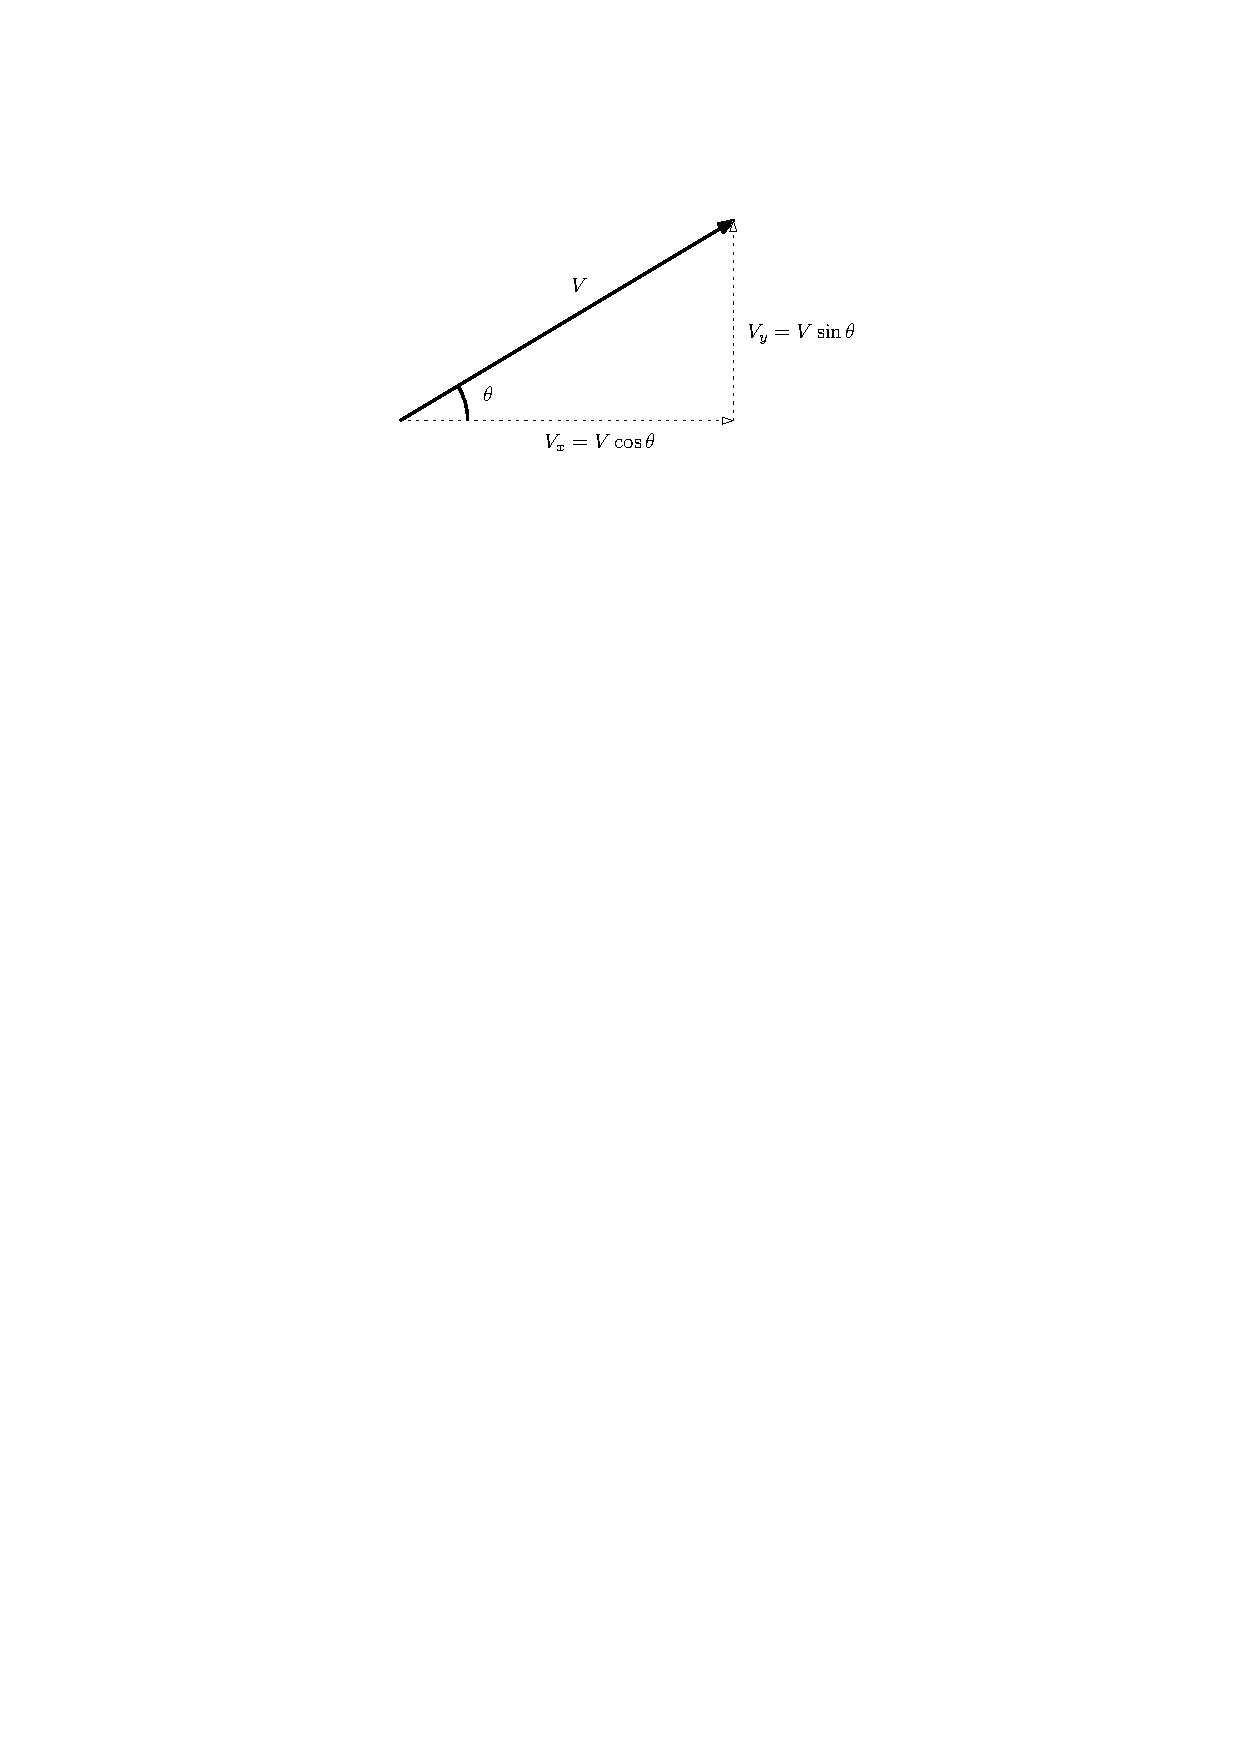
\includegraphics{vecComps} \hfill \mbox{}

\vspace{1cm}

\hspace{2cm} \parbox{9cm}{For example, to add $A = (10 \un, \hspace{.1cm} 35^{\circ})$ and  $B = (15 \un, \hspace{.1cm} 100^{\circ})$, first find the $x$ and $y$ components of each: $$A_x = 8.19 \un \hspace{1cm} A_y = 5.74 \un$$ $$B_x =-2.60 \un \hspace{1cm} B_y = 14.77 \un$$}

\vspace{.1cm}

\hfill 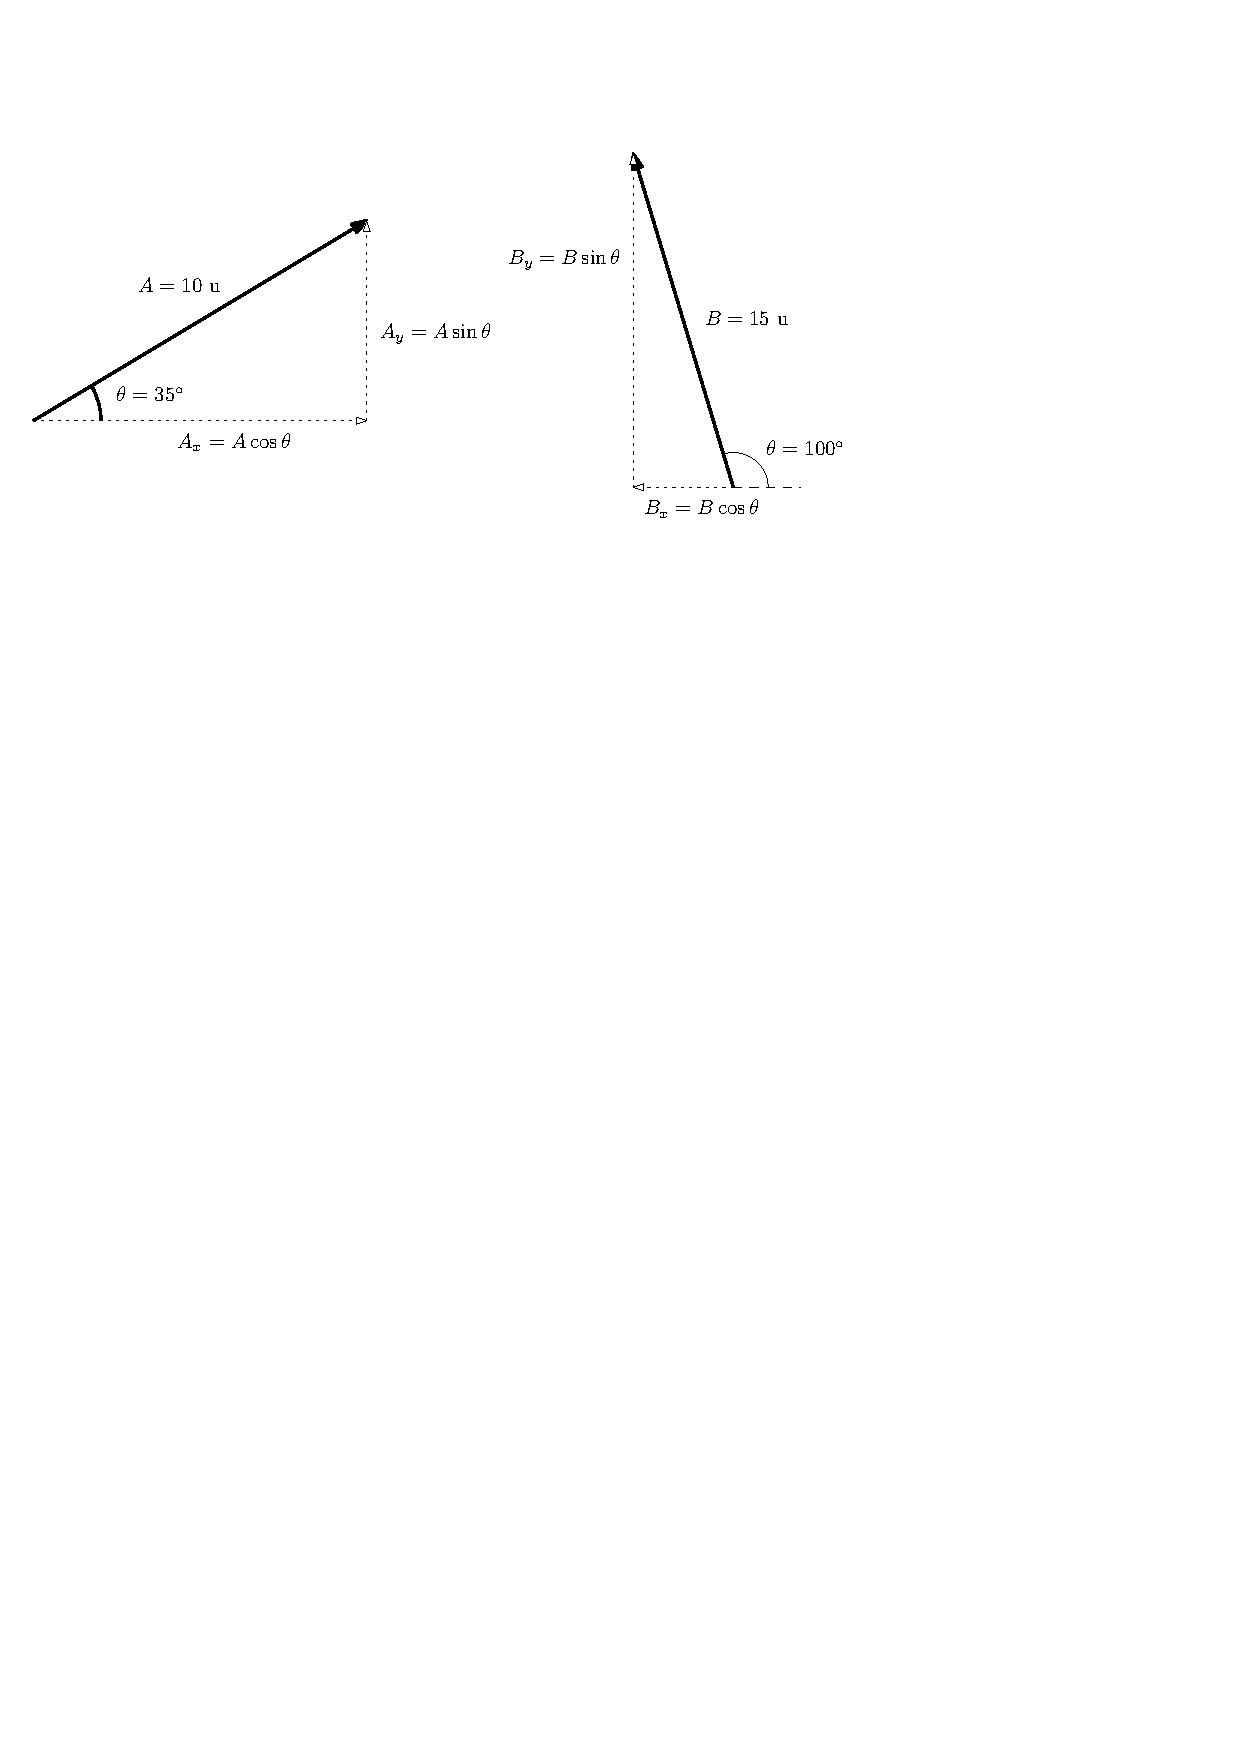
\includegraphics{vectors_35plus100} \hspace{3cm}

\hspace{2cm} \parbox{6cm}{$$R_x = A_x+B_x = 5.59 \un$$ $$R_y = A_y + B_y = 20.51 \un$$ $$R = \sqrt{(R_x)^2 + (R_y)^2} = 21.26 \un$$ $$\theta = \tan^{-1}(\frac{R_y}{R_x}) = 74.75^{\circ}$$} \hfill \parbox{6cm}{The magnitude of the resultant vector, $R$, is found by adding components and using the pythagorean theorem.  The angle is found by using inverse tangent.} \hspace{2cm}

\vfill

\hfill Try adding $A = (5 \un, \hspace{.1cm} 25^{\circ})$ and  $B = (7 \un, \hspace{.1cm} 75^{\circ})$ \hfill [Ans: $A+B =  (10.90 \un, \hspace{.1cm} 54.44^{\circ} = )$] \hfill \mbox{}

\end{document}